% Misión 3: entrega a domicilio. Portada y vuelo paso a paso.
% NED: la farmacia (despegue, H) en 0,0; la casa destino (~9 m de alto) en N 25, E 16;
% la plataforma del patio en N 36, E 16.

\begin{frame}{Misión 3: entrega a domicilio}
  \begin{columns}[c]
    \column{0.56\textwidth}
    \begin{tikzpicture}
      \node[inner sep=0] (im) {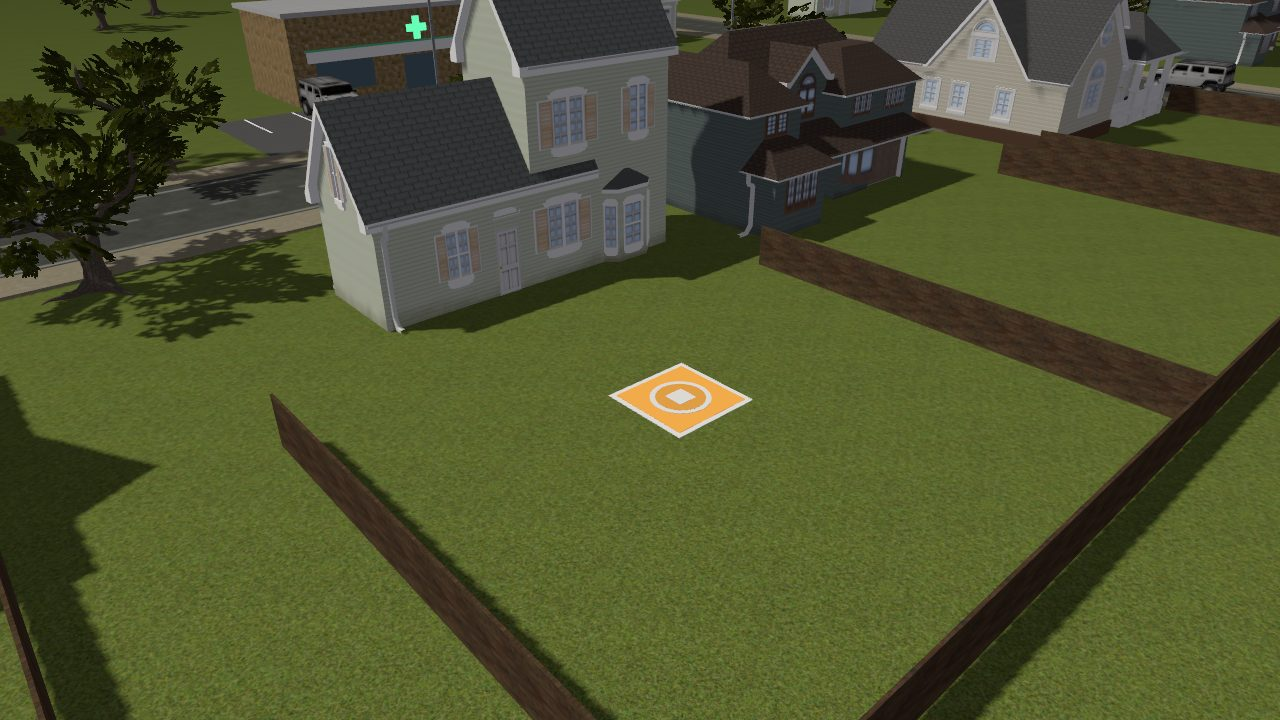
\includegraphics[width=\linewidth]{barrio_entrega_patio}};
      \node[anchor=north west,fill=azul,text=white,font=\bfseries\scriptsize,rounded corners=2pt]
        at ([xshift=4pt,yshift=-4pt]im.north west) {MISIÓN 3 · NIVEL 1 \nivel{1}};
    \end{tikzpicture}\\[0.3em]
    \small\textbf{Escenario}: llevar un medicamento de la farmacia a la plataforma naranja en el patio de una
    casa, a \textasciitilde40 m; dejarlo y \textbf{volver solo}.
    \column{0.41\textwidth}
    \ficha{x500_volando}{x500}{barrio\_entrega}{entrega\_domicilio}{\cmd{goto\_mission}, \cmd{return\_home},
      \cmd{set\_home}}{\textbf{sin offboard}: PX4 vuela, tu nodo decide qué sigue}{termina a \textless 1.5 m de la H
      de la farmacia}
  \end{columns}
\end{frame}

\begin{frame}{La entrega, paso a paso}
  \begin{columns}[c]
    \column{0.45\textwidth}\centering
    \begin{tikzpicture}[scale=0.1]
      \draw[gray!20,step=5] (-12,-16) grid (32,44);
      \fill[gray!25] (-12,4) rectangle (32,14); \node[font=\tiny,text=gris] at (25,9) {calle};
      \draw[fill=red!25,draw=red!50] (-9,-15) rectangle (9,-7); \node[font=\tiny] at (0,-11) {farmacia};
      \draw[fill=orange!25,draw=orange!60] (10,20) rectangle (22,30); \node[font=\tiny,align=center] at (16,25) {casa\\(9 m)};
      \fill[orange] (14.5,34.5) rectangle (17.5,37.5); \node[font=\tiny,right] at (18,36) {patio};
      \node[draw,circle,fill=azulclaro,inner sep=0.3pt,font=\tiny] at (0,0) {H};
      \draw[-{Stealth},verde,thick] (-10,-4) -- (-10,2) node[above,font=\tiny] {N};
      % ida y vuelta
      \draw[azul,line width=1.5pt,visible on=<4->] (0,0) -- (16,36);
      \draw[azul,dashed,thick,-{Stealth},visible on=<3>] (1,2.3) -- (15,33.7);
      \draw[naranja,dashed,thick,-{Stealth},visible on=<7>] (15,33.7) -- (1,2.3);
      \only<1-3,8>{\node at (0,0) {\dronarriba{0.8cm}};}
      \only<4-7>{\node at (16,36) {\dronarriba{0.8cm}};}
      \only<6>{\node[draw=rojo,fill=red!10,font=\tiny,align=center,rounded corners] at (16,43) {¡casa = aquí!};}
      \only<7->{\node[draw=verde,fill=verdeclaro,font=\tiny,rounded corners] at (6,-4) {casa = farmacia};}
    \end{tikzpicture}
    \column{0.08\textwidth}\centering
    \begin{tikzpicture}[y=0.1cm]
      \draw[gray] (0,0) -- (0,32); \node[font=\tiny,text=gris] at (0,35) {altura};
      \foreach \h in {0,15,30} \draw[gray] (-0.12,\h) -- (0.12,\h) node[right,font=\tiny,text=gris] {\h};
      \only<1,4-5,8>{\fill[azul] (0,0) circle (4pt);}
      \only<2,6>{\draw[-{Stealth},line width=2pt,verde] (0,1) -- (0,14);}
      \only<3>{\fill[azul] (0,15) circle (4pt);}
      \only<7>{\fill[naranja] (0,30) circle (4pt);}
    \end{tikzpicture}
    \column{0.45\textwidth}
    \only<1>{\begin{terminal}{entrega\_domicilio}
entrega\_domicilio: esperando GPS...\\
{[}1/9] GPS listo. Destino a 39.4 m. Armando
    \end{terminal}\small Guarda dónde está la farmacia y arma (con comandos, no offboard).}%
    \only<2>{\begin{terminal}{entrega\_domicilio}
{[}2/9] Despegando a 15 m
    \end{terminal}\small \cmd{NAV\_TAKEOFF}. 15 m: más alto que la casa que está en el camino.}%
    \only<3>{\begin{terminal}{entrega\_domicilio}
{[}3/9] A la altura, volando al patio\\
\ \ \ \ \ \ faltan 21.4 m
    \end{terminal}\small \cmd{DO\_REPOSITION} a la latitud y longitud del patio. PX4 vuela solo.}%
    \only<4>{\begin{terminal}{entrega\_domicilio}
{[}4/9] Sobre el patio, aterrizando
    \end{terminal}\small \cmd{NAV\_LAND}: baja a la plataforma y desarma.}%
    \only<5>{\begin{terminal}{entrega\_domicilio}
{[}5/9] En el patio (a 0.21 m de la plataforma).\\
\ \ Entregando...\\
TODO: la vuelta a casa no está hecha todavía
    \end{terminal}\small Hasta aquí ya funciona. \textbf{De aquí en adelante es tu parte}: esperar
      \cmd{wait} (5 s) desarmado, como si soltara el paquete.}%
    \only<6>{\small\textbf{Tu parte}: volver a armar y despegar.
      \begin{ojo}[title={\small\bfseries La trampa}]
        \small PX4 pone ``casa'' \textbf{donde arma}. Ahora casa es el patio: un Return se quedaría aquí.
      \end{ojo}}%
    \only<7>{\small\textbf{Tu parte}: \cmd{set\_home\_to\_pharmacy()}, esperar a que PX4 lo acepte
      (\cmd{home().update\_count} sube) y luego \textbf{Return}: sube a 30 m, vuela a la farmacia y baja.}%
    \only<8>{\begin{terminal}{entrega\_domicilio}
De vuelta en la farmacia y desarmado. Misión de 119 s\\
\ \ a 0.01 m de la H OK\\
Misión cumplida
    \end{terminal}}%
  \end{columns}
\end{frame}
